\documentclass[12pt,a4paper,oneside]{article}

\usepackage[utf8]{inputenc}
\usepackage[T1]{fontenc}
\usepackage[ngerman]{babel}
\usepackage{geometry}
\usepackage{graphicx}
\usepackage{float}
\usepackage{booktabs}
\usepackage{tabularx}
\usepackage{array}
\usepackage{enumitem}
\usepackage{xcolor}
\usepackage{fancyhdr}
\usepackage{hyperref}

\geometry{left=24mm,right=24mm,top=25mm,bottom=25mm}
\graphicspath{{images/}}
\setlength{\parindent}{0pt}
\setlength{\parskip}{5pt}
\emergencystretch=2em
\setcounter{tocdepth}{2}
\setcounter{secnumdepth}{2}

\hypersetup{
    colorlinks=true,
    linkcolor=black,
    urlcolor=blue,
    pdftitle={Designdokument -- SSM-Demonstrator},
    pdfauthor={Gruppe 3}
}

\pagestyle{fancy}
\fancyhf{}
\lhead{Designdokument -- SSM-Demonstrator}
\rhead{Gruppe 3}
\cfoot{\thepage}
\setlength{\headheight}{15pt}

% Hilfsmakros
\newcommand{\keybox}[1]{%
    \begin{center}
        \fbox{\parbox{0.86\textwidth}{\centering\textbf{#1}}}
    \end{center}}
\newcommand{\hazfield}[1]{\par\medskip\noindent\textbf{#1:}\enspace}
\newcommand{\failsafe}[1]{\keybox{#1}}
\newcommand{\hazop}[1]{\par\smallskip\noindent\textbf{HAZOP Guide Words:} #1\par}
\newcolumntype{Y}{>{\raggedright\arraybackslash}X}

\begin{document}

\begin{titlepage}
	% No header
	\thispagestyle{empty} 
	
	\begin{picture}(50,50)
		\put(-70,40){\hbox{\includegraphics{images/header.png}}}
	\end{picture}
	
	%\vspace*{-5.8cm}
	
	\vspace*{2cm}
	
	\begin{center}
		{\LARGE\bfseries Designdokument\par}
		\vspace{0.5cm}
		{\Large Geschwindigkeitsabhängiges Schutzsystem\par}
		\vspace{0.25cm}
		{\large Safety- und Security-Demonstrator mit rotierendem Aktor\par}
		
		\vfill
		
		{\large\textbf{Gruppe 3}\par}
		\vspace{0.7cm}
		Andreas Günter Kostecka\\
		Jonas Gök\\
		Loïc Thill\\
		David Freudenthaler
		
		\vfill
		
		{\large FH Campus Wien\par}
		\vspace{0.3cm}
		{\large Stand: \today\par}
	\end{center}
\end{titlepage}
\tableofcontents
\newpage

\section{Projektbeschreibung}
\label{sec:project}

\subsection{Ziel und Systemidee}

Ziel des Projekts ist ein Demonstrator für ein geschwindigkeitsabhängiges
Schutzsystem eines rotierenden Aktors. Das Prinzip orientiert sich vereinfacht
an \emph{Speed and Separation Monitoring} (SSM): Mit steigender
Geschwindigkeitsstufe wird ein größerer Sicherheitsabstand verwendet.
Unterschreitet ein Objekt diesen Abstand, wird die Motoransteuerung abgeschaltet.

Der Demonstrator dient ausschließlich zur Untersuchung eines
sicherheitsgerichteten Prinzips. Er ist kein zertifiziertes Safety-System.
Insbesondere werden Raspberry Pi 4B, HC-SR04, Bluetooth und der verwendete
Motortreiber nicht als Safety-zertifizierte Komponenten betrachtet.

\keybox{Sicherer Zustand: Motor AUS -- der Rotor wird nicht aktiv angetrieben.}

Ein Software-Stopp bedeutet nicht automatisch mechanischen Stillstand. Der Rotor
kann aufgrund seiner Massenträgheit nachlaufen. Diese Nachlaufzeit muss bei der
Festlegung der Sicherheitsabstände berücksichtigt werden.

\subsection{Systemaufbau}

Das System besteht aus zwei Raspberry Pi 4B, zwei Ultraschall-Abstandssensoren
HC-SR04, einem Elektromotor mit Rotor, einem Motortreiber, einem LCD-Display und
einer Bluetooth-Verbindung zwischen den Raspberry Pis.

\begin{table}[H]
    \centering
    \small
    \begin{tabularx}{\textwidth}{@{}p{3.7cm}YY@{}}
        \toprule
        \textbf{Komponente} & \textbf{Aufgabe} & \textbf{Bedeutung für Safety} \\
        \midrule
        Raspberry Pi 1 & Bedienung, Auswahl der Geschwindigkeitsstufe, LCD-Anzeige, Logging und Bluetooth-Kommunikation & Liefert Sollwerte und zeigt Zustände an. LCD und Logging sind keine Safety-Funktionen. \\
        Raspberry Pi 2 & Sensorerfassung, Plausibilitätsprüfung, Safety-Logik und Motorsteuerung & Führt die lokale Safety-Entscheidung aus und kann den Motor unabhängig von Pi 1 abschalten. \\
        2 $\times$ HC-SR04 & Abstandsmessung zum Gefahrenbereich & Zwei gleiche Sensoren ermöglichen einen Quervergleich, bilden aber keine nachgewiesene Safety-Redundanz. \\
        Motortreiber / Motor & Umsetzung der Motoransteuerung und rotierende Gefahrenquelle & Motor AUS entspricht PWM = 0 und deaktiviertem Enable-Signal. Mechanischer Stillstand ist dadurch nicht garantiert. \\
        Bluetooth & Bidirektionale Kommunikation zwischen Pi 1 und Pi 2 & Wird mit Heartbeat, Timeout und Plausibilitätsprüfungen überwacht. \\
        \bottomrule
    \end{tabularx}
    \caption{Komponenten und Aufgaben des Demonstrators}
\end{table}

\subsection{Funktionsablauf}

Nach dem Start initialisieren beide Raspberry Pis ihre benötigten Schnittstellen
und Threads. Raspberry Pi 2 hält die Motoransteuerung während der
Initialisierung im sicheren Zustand. Erst wenn gültige Sensordaten, eine gültige
Kommunikation und eine gültige Geschwindigkeitsstufe vorliegen, darf der Motor
freigegeben werden.

Raspberry Pi 1 sendet die gewünschte Geschwindigkeitsstufe
\texttt{LOW}, \texttt{MEDIUM} oder \texttt{HIGH} sowie einen Heartbeat an
Raspberry Pi 2. Raspberry Pi 2 liest beide Abstandssensoren aus, prüft die
Messwerte und wählt den zugehörigen Sicherheitsabstand. Befindet sich ein Objekt
innerhalb dieses Abstands oder schlägt eine Safety-Prüfung fehl, wird der Motor
abgeschaltet.

Raspberry Pi 2 sendet Status, Abstandswerte und Fehlermeldungen an Raspberry Pi
1 zurück. Diese Informationen werden am LCD angezeigt und protokolliert.

Nach einer Abschaltung läuft der Motor ohne Quittierung wieder an, sobald alle
Prüfungen bestanden sind (Wiederanlaufbedingung, siehe
Abschnitt~\ref{sec:states}).

\subsection{Zentrale Designparameter}

Die folgenden Werte sind Projektparameter für den Demonstrator und müssen am
realen Aufbau getestet und gegebenenfalls angepasst werden.

\begin{table}[H]
    \centering
    \begin{tabularx}{\textwidth}{@{}p{5.1cm}p{3.2cm}Y@{}}
        \toprule
        \textbf{Parameter} & \textbf{Startwert} & \textbf{Bedeutung} \\
        \midrule
        Heartbeat Pi 1 $\rightarrow$ Pi 2 & 100 ms (10 Hz) & Zyklische Lebensmeldung und Übertragung der Sollstufe \\
        Kommunikations-Timeout & 300 ms & Keine gültige Nachricht innerhalb dieses Zeitraums führt zu Motor AUS \\
        Safety-Logik-Zyklus & 50 ms & Zyklische Prüfung der Safety-Bedingungen auf Pi 2 \\
        Max. Alter der Sensordaten & 150 ms & Ältere Messwerte dürfen nicht für eine Freigabe verwendet werden \\
        Gültiger Messbereich & 2--400 cm & Werte außerhalb des Messbereichs des HC-SR04 sind ungültig \\
        Max. Abstandsänderung & 0{,}2 cm/ms (= 2 m/s) & Schnellere Änderung zwischen zwei Messungen eines Sensors ist unplausibel \\
        Sensorabweichung & $> 5$ cm in zwei aufeinanderfolgenden Messzyklen & Sensorwerte werden als unplausibel bewertet \\
        Sicherheitsabstände & $S_{\mathrm{LOW}} < S_{\mathrm{MEDIUM}} < S_{\mathrm{HIGH}}$ & Endgültige Werte werden am Demonstrator anhand von Reaktions- und Nachlaufzeit festgelegt \\
        \bottomrule
    \end{tabularx}
    \caption{Zentrale Startwerte des Designs}
\end{table}

\subsection{Grenzen des Demonstrators}
\label{sec:limits}

Die tatsächliche Motordrehzahl wird nicht mit einem Encoder gemessen. Daher darf
nicht angenommen werden, dass ein PWM-Wert proportional zur realen Drehzahl ist.
Die Geschwindigkeitsstufen stellen lediglich definierte Ansteuerungsklassen dar.
Außerdem können zwei gleiche HC-SR04 durch eine gemeinsame Fehlerursache
ähnliche falsche Werte liefern. Ein Defekt des Motortreibers, bei dem der Motor
trotz Abschaltsignal weiter bestromt wird, kann mit der vorhandenen Architektur
nicht sicher beherrscht werden.

Der Wiederanlauf erfolgt automatisch, ohne Quittierung durch den Bediener.
Nach einem Fehler oder einem Objekt-Stopp kann der Motor daher wieder anlaufen,
ohne dass der Bediener dies ausdrücklich freigegeben hat. Befindet sich ein
Objekt genau an der Grenze des Sicherheitsabstands, kann der Motor
wiederholt ein- und ausschalten. Diese Einschränkungen werden für den
Demonstrator bewusst akzeptiert. In einer industriellen Anwendung wäre ein
unerwarteter Wiederanlauf durch eine Quittierung und eine Hysterese zu
verhindern.

\clearpage
\section{Softwarearchitektur und Design}
\label{sec:software}

Die Software wird in C unter Linux auf beiden Raspberry Pis implementiert.
Threads werden verwendet, um Sensorerfassung, Kommunikation, Bedienung und
Safety-Logik voneinander zu trennen. Safety-relevante Entscheidungen werden auf
Raspberry Pi 2 getroffen; ein Ausfall von LCD oder Logging darf die
Motorabschaltung nicht verhindern.

\subsection{Raspberry Pi 1 -- Host und Bedienung}

\begin{table}[H]
    \centering
    \small
    \begin{tabularx}{\textwidth}{@{}p{4.2cm}Y@{}}
        \toprule
        \textbf{Modul / Thread} & \textbf{Aufgabe} \\
        \midrule
        Initialisierung & Bluetooth, LCD, Logging und benötigte Threads starten \\
        UI / Eingabe & Geschwindigkeitsstufe \texttt{LOW}, \texttt{MEDIUM}, \texttt{HIGH} auswählen und Programmende anfordern \\
        Kommunikations-/Heartbeat-Thread & Sollstufe und Heartbeat alle 100 ms senden; Status und Fehlermeldungen von Pi 2 empfangen \\
        Anzeige & Systemzustand, Geschwindigkeitsstufe, kleinsten gemessenen Abstand $d_{\min}$ und Fehlercode am LCD anzeigen (siehe Abschnitt~\ref{sec:distances}) \\
        Logging & Ereignisse sofort und Messwerte mit 10 Hz protokollieren (siehe Abschnitt~\ref{sec:logging}); keine Safety-Funktion \\
        \bottomrule
    \end{tabularx}
    \caption{Softwareaufgaben auf Raspberry Pi 1}
\end{table}

\subsection{Raspberry Pi 2 -- Steuerung und Überwachung}

\begin{table}[H]
    \centering
    \small
    \begin{tabularx}{\textwidth}{@{}p{4.2cm}Y@{}}
        \toprule
        \textbf{Modul / Thread} & \textbf{Aufgabe} \\
        \midrule
        Initialisierung & Motor sicher deaktivieren, Sensoren, Bluetooth und Threads initialisieren \\
        Sensor-Thread 1 / 2 & HC-SR04 auslesen; Messbereich und Abstandsänderung prüfen; Messwert, Gültigkeitsstatus und Zeitstempel bereitstellen \\
        Kommunikations-Thread & Nachrichten von Pi 1 empfangen und prüfen; Heartbeat-Timeout überwachen; Status alle 100 ms an Pi 1 senden \\
        Safety-Logik-Thread & Zyklisch alle 50 ms Sensorplausibilität, Kommunikation und Datenaktualität prüfen; Sicherheitsabstand auswählen und Motorfreigabe entscheiden \\
        Motorsteuerungs-Thread & Motorstufe setzen oder Motor mit PWM = 0 und Enable = OFF abschalten \\
        \bottomrule
    \end{tabularx}
    \caption{Softwareaufgaben auf Raspberry Pi 2}
\end{table}

\subsection{Safety-Logik-Thread}

Der Safety-Logik-Thread ist ein eigener Thread auf Raspberry Pi 2. Er führt
keine blockierenden Netzwerk- oder Logging-Aufrufe aus. In jedem Zyklus werden
folgende Prüfungen in dieser Reihenfolge ausgeführt:

\begin{enumerate}
    \item Wurde ein Stop/Shutdown-Befehl empfangen?
    \item Sind beide Sensorwerte gültig und zueinander plausibel?
    \item Ist die Kommunikation aktuell und der empfangene Befehl gültig?
    \item Sind die verwendeten Sensordaten noch aktuell?
    \item Welcher Sicherheitsabstand gehört zur gültigen Geschwindigkeitsstufe?
    \item Liegt der aktuelle Abstand innerhalb des Sicherheitsabstands?
\end{enumerate}

Wurde ein Stop/Shutdown-Befehl empfangen, wird der Motor abgeschaltet und das
Programm kontrolliert beendet. Schlägt eine der Prüfungen 2 bis 4 fehl, wird ein
Fehlerzustand gesetzt und die Motoransteuerung deaktiviert. Erst wenn alle Prüfungen erfolgreich sind,
darf die normale Motorsteuerung ausgeführt werden.

\subsection{Verwendete Abstände}
\label{sec:distances}

Die Abstandsüberwachung verwendet folgende Größen:

\begin{table}[H]
    \centering
    \small
    \begin{tabularx}{\textwidth}{@{}p{3.6cm}Y@{}}
        \toprule
        \textbf{Größe} & \textbf{Bedeutung} \\
        \midrule
        $d_1$, $d_2$ & Gemessene Abstände von Sensor 1 und Sensor 2. Beide werden benötigt, um die Sensoren gegeneinander zu prüfen (P3). \\
        $d_{\min} = \min(d_1, d_2)$ & Kleinerer der beiden gültigen Messwerte. Er wird für die Abschaltentscheidung verwendet, weil er den ungünstigeren Fall darstellt. \\
        $S_{\mathrm{LOW}}$, $S_{\mathrm{MEDIUM}}$, $S_{\mathrm{HIGH}}$ & Sicherheitsabstand je Geschwindigkeitsstufe. Bei höherer Stufe sind Nachlaufzeit und zurückgelegter Weg des Rotors größer, deshalb gilt $S_{\mathrm{LOW}} < S_{\mathrm{MEDIUM}} < S_{\mathrm{HIGH}}$. \\
        $S$ & Aktiver Sicherheitsabstand, also der Wert, der zur aktuell gültigen Geschwindigkeitsstufe gehört. Der Motor wird abgeschaltet, wenn $d_{\min} < S$. \\
        \bottomrule
    \end{tabularx}
    \caption{Begriffe der Abstandsüberwachung}
\end{table}

Am LCD wird nur $d_{\min}$ angezeigt. $d_1$ und $d_2$ werden einzeln
protokolliert, damit Abweichungen zwischen den Sensoren nachvollziehbar sind.

\subsection{Plausibilitätsprüfung der Sensorwerte}
\label{sec:plausibility}

Ein Sensorwert wird nur verwendet, wenn er die Prüfungen P1--P4 besteht. Die
Prüfungen P1 und P2 betreffen jeden Sensor einzeln und werden im jeweiligen
Sensor-Thread durchgeführt. Das Ergebnis wird als Gültigkeitsstatus im
Datensatz abgelegt. P3 und P4 vergleichen bzw. bewerten die Daten und werden im
Safety-Logik-Thread durchgeführt.

\begin{table}[H]
    \centering
    \small
    \begin{tabularx}{\textwidth}{@{}p{0.7cm}p{3.1cm}Yp{2.3cm}@{}}
        \toprule
        \textbf{ID} & \textbf{Prüfung} & \textbf{Bedingung für „ungültig“} & \textbf{Ort} \\
        \midrule
        P1 & Messbereich & $d < 2$ cm oder $d > 400$ cm (Grenzen des HC-SR04). Bleibt das Echo aus (Timeout), wird der Messwert ebenfalls als ungültig markiert. & Sensor-Thread \\
        P2 & Abstandsänderung & $\frac{|d_k - d_{k-1}|}{t_k - t_{k-1}} > 0{,}2$ cm/ms, also eine Änderung schneller als 2 m/s zwischen zwei Messungen desselben Sensors. & Sensor-Thread \\
        P3 & Quervergleich & $|d_1 - d_2| > 5$ cm in zwei aufeinanderfolgenden Messzyklen. & Safety-Logik \\
        P4 & Datenalter & Messwert älter als 150 ms. & Safety-Logik \\
        \bottomrule
    \end{tabularx}
    \caption{Plausibilitätsprüfungen der Abstandssensoren}
\end{table}

Die Grenze von 2 m/s in P2 entspricht der Annäherungsgeschwindigkeit, die die
EN ISO 13855 für Handbewegungen ansetzt. P2 filtert vor allem Ausreißer und
Sprünge des Messwerts. Taucht ein Objekt seitlich im Messbereich auf oder nähert
es sich schneller, kann der Messwert ebenfalls sprunghaft kleiner werden und P2
auslösen. Die Reaktion ist in allen Fällen Motor AUS und liegt damit auf der
sicheren Seite.

\subsection{Systemzustände}
\label{sec:states}

Raspberry Pi 2 befindet sich immer in genau einem der folgenden Zustände. Der
aktuelle Zustand wird im Status an Pi 1 übertragen und am LCD angezeigt.

\begin{table}[H]
    \centering
    \small
    \begin{tabularx}{\textwidth}{@{}p{2.7cm}p{2.2cm}Y@{}}
        \toprule
        \textbf{Zustand} & \textbf{Motor} & \textbf{Bedeutung} \\
        \midrule
        \texttt{INIT} & AUS & Programmstart; Schnittstellen und Threads werden initialisiert. Noch keine Safety-Bewertung. \\
        \texttt{BETRIEB} & AN (\texttt{LOW}, \texttt{MEDIUM} oder \texttt{HIGH}) & Alle Prüfungen bestanden und $d_{\min} \geq S$. \\
        \texttt{OBJEKT\_STOPP} & AUS & Alle Prüfungen bestanden, aber $d_{\min} < S$. Kein Fehler, sondern bestimmungsgemäße Schutzreaktion. \\
        \texttt{FEHLER} & AUS & Mindestens eine Prüfung fehlgeschlagen. Ein Fehlercode gibt die Ursache an: \texttt{SENSOR} (P1--P3), \texttt{KOMMUNIKATION} (Timeout oder ungültiger Befehl), \texttt{DATENALTER} (P4). \\
        \texttt{SHUTDOWN} & AUS & Stop/Shutdown-Befehl empfangen; Threads werden kontrolliert beendet. Endzustand. \\
        \bottomrule
    \end{tabularx}
    \caption{Systemzustände von Raspberry Pi 2}
\end{table}

\texttt{INIT} wird nach Abschluss der Initialisierung verlassen. Danach wird der
Zustand in jedem Zyklus des Safety-Logik-Threads neu aus den Prüfergebnissen
bestimmt, in derselben Reihenfolge wie im Flussdiagramm
(Abbildung~\ref{fig:flowchart}):

\begin{enumerate}
    \item Stop/Shutdown empfangen $\rightarrow$ \texttt{SHUTDOWN}
    \item Eine der Prüfungen Sensorplausibilität, Kommunikation oder Datenaktualität fehlgeschlagen $\rightarrow$ \texttt{FEHLER}
    \item $d_{\min} < S$ $\rightarrow$ \texttt{OBJEKT\_STOPP}
    \item sonst $\rightarrow$ \texttt{BETRIEB}
\end{enumerate}

\textbf{Wiederanlaufbedingung:} Der Zustand \texttt{FEHLER} ist nicht selbsthaltend. Aus
\texttt{FEHLER} oder \texttt{OBJEKT\_STOPP} geht das System in \texttt{BETRIEB}
über, sobald in einem Zyklus alle folgenden Bedingungen gleichzeitig erfüllt
sind:

\begin{itemize}
    \item kein Stop/Shutdown-Befehl empfangen,
    \item beide Sensorwerte gültig und zueinander plausibel (P1--P3),
    \item gültige Nachricht von Pi 1 innerhalb der letzten 300 ms mit gültiger Geschwindigkeitsstufe,
    \item Sensordaten nicht älter als 150 ms (P4),
    \item $d_{\min} \geq S$ für die aktuell gültige Stufe.
\end{itemize}

Die Motorstufe wird dann im selben Zyklus freigegeben, und der Motor läuft mit
der von Pi 1 angeforderten Stufe an. Eine Quittierung durch den Bediener
ist nicht vorgesehen; die daraus folgenden Einschränkungen sind in
Abschnitt~\ref{sec:limits} beschrieben.

Auf Pi 1 wird zusätzlich „Verbindung getrennt“ angezeigt, wenn länger
als 300 ms kein gültiger Status von Pi 2 empfangen wurde. Der zuletzt
empfangene Zustand wird dann nicht mehr als aktuell dargestellt.

\subsection{Gemeinsam verwendete Daten}
\label{sec:shared}

Sensor- und Kommunikations-Threads aktualisieren Daten, die vom
Safety-Logik-Thread gelesen werden. Damit keine Race Conditions entstehen,
werden zusammengehörige Werte als Datensatz behandelt, zum Beispiel:

\begin{verbatim}
struct sensor_data {
    float distance_cm;
    bool valid;
    struct timespec timestamp;
};
\end{verbatim}

Der schreibende Thread aktualisiert den vollständigen Datensatz geschützt durch
einen Mutex. Der Safety-Logik-Thread kopiert den Datensatz unter demselben Mutex
in eine lokale Variable und arbeitet anschließend nur mit diesem Snapshot.
Zeitmessungen für Timeouts und Datenalter erfolgen mit der monotonen Uhr
\texttt{CLOCK\_MONOTONIC} (siehe Abschnitt~\ref{subsec:security-addressed}, T3).

Konkret werden folgende gemeinsamen Datensätze verwendet:

\begin{table}[H]
    \centering
    \small
    \begin{tabularx}{\textwidth}{@{}p{3.2cm}p{3.0cm}p{3.0cm}Y@{}}
        \toprule
        \textbf{Datensatz} & \textbf{Schreibt} & \textbf{Liest} & \textbf{Inhalt} \\
        \midrule
        \texttt{sensor\_data[2]} & Sensor-Thread 1 / 2 & Safety-Logik, Kommunikation & Abstand, Gültigkeit (P1, P2), Zeitstempel \\
        \texttt{comm\_data} & Kommunikations-Thread & Safety-Logik & Sollstufe, Stop-Flag, Zeitstempel der letzten gültigen Nachricht \\
        \texttt{safety\_state} & Safety-Logik & Kommunikation, Motorsteuerung & Systemzustand, Fehlercode, freigegebene Motorstufe \\
        \bottomrule
    \end{tabularx}
    \caption{Gemeinsame Datensätze auf Raspberry Pi 2}
\end{table}

Für die Umsetzung gelten folgende Regeln:

\begin{itemize}
    \item Jeder Datensatz hat genau einen schreibenden Thread und einen eigenen \texttt{pthread\_mutex\_t}.
    \item Die Mutexe werden mit dem Protokoll \texttt{PTHREAD\_PRIO\_INHERIT} angelegt, damit ein niedriger priorisierter Thread den Safety-Logik-Thread nicht durch Prioritätsinversion aufhält.
    \item Unter einem Mutex wird nur kopiert. Messungen, Bluetooth-Zugriffe, Logging und GPIO-Zugriffe erfolgen außerhalb des gesperrten Bereichs.
    \item Ein Thread hält immer nur einen Mutex gleichzeitig; dadurch sind Deadlocks ausgeschlossen.
    \item Der Safety-Logik-Thread läuft mit \texttt{SCHED\_FIFO} und der höchsten Priorität der Anwendung.
    \item Nur der Safety-Logik-Thread schreibt die freigegebene Motorstufe. Die Motorsteuerung setzt ausschließlich diesen Wert um.
\end{itemize}

\subsection{Bluetooth-Kommunikation}
\label{sec:bt}

Die Kommunikation ist bidirektional. Raspberry Pi 1 sendet Sollstufe,
Heartbeat, Sequenznummer und gegebenenfalls einen Stop/Shutdown-Befehl.
Raspberry Pi 2 sendet Status, aktuelle Abstandswerte und Fehlermeldungen zurück.

Bevor die Nutzdaten gelesen werden, prüft Pi 2, ob die Länge zum
Nachrichtentyp passt. Ein unbekannter Typ oder eine falsche Länge führt zum
Abbau der Verbindung, da der Datenstrom danach nicht mehr synchron ist. Nach dem
Einlesen prüft Pi 2 zuerst das GCM-Tag, danach Session-ID, Sequenznummer und
Wertebereich der Nutzdaten. Schlägt eine dieser Prüfungen fehl, wird die
Nachricht verworfen. Bleibt eine gültige Nachricht länger als
300 ms aus, wird die Kommunikation als fehlerhaft bewertet und der Motor
abgeschaltet.

\textbf{Umsetzung der Datenübertragung:}

\begin{itemize}
    \item Die Verbindung wird als RFCOMM-Socket über die BlueZ-Socket-API aufgebaut (\texttt{AF\_BLUETOOTH}, \texttt{SOCK\_STREAM}, \texttt{BTPROTO\_RFCOMM}). Pi 2 ist Server und wartet auf einem festen Kanal, Pi 1 ist Client. Die beiden Geräte werden einmalig gekoppelt. Nach dem Verbindungsaufbau sendet Pi 2 zuerst eine \texttt{STATUS}-Nachricht mit einer neuen Session-ID; erst danach beginnt Pi 1 mit den Heartbeats (siehe Abschnitt~\ref{subsec:security-addressed}, T2).
    \item Da RFCOMM einen Datenstrom und keine einzelnen Pakete liefert, beginnt jede Nachricht mit einem Typ- und einem Längenfeld. Der Empfänger liest zuerst diese Felder und danach genau die angegebene Anzahl Bytes.
    \item Nachrichten werden Feld für Feld in ein Byte-Array in Big-Endian-Reihenfolge (Network Byte Order, umgesetzt mit \texttt{htons()} und \texttt{htonl()}) geschrieben, nicht als C-\texttt{struct} kopiert. Dadurch spielen Padding und Compiler-Unterschiede keine Rolle.
    \item Abstände werden als ganze Millimeter (\texttt{uint16\_t}) übertragen, Stufen, Zustände und Fehlercodes als \texttt{uint8\_t} mit festgelegten Werten. Unbekannte Werte führen zum Verwerfen der Nachricht.
    \item Der Kommunikations-Thread wartet mit \texttt{poll()} und einem Timeout von 50 ms auf Daten. Er blockiert dadurch nie dauerhaft und kann den Heartbeat-Timeout auch dann auswerten, wenn keine Daten ankommen.
    \item Bricht die Verbindung ab, versucht Pi 1 jede Sekunde, sie neu aufzubauen. Pi 2 bleibt währenddessen über den Kommunikations-Timeout im Zustand \texttt{FEHLER}.
\end{itemize}

\begin{table}[H]
    \centering
    \small
    \begin{tabularx}{\textwidth}{@{}p{2.6cm}p{2.3cm}p{2.0cm}Y@{}}
        \toprule
        \textbf{Nachricht} & \textbf{Richtung} & \textbf{Takt} & \textbf{Nutzdaten} \\
        \midrule
        \texttt{HEARTBEAT} & Pi 1 $\rightarrow$ Pi 2 & 100 ms & Sollstufe \\
        \texttt{STOP} & Pi 1 $\rightarrow$ Pi 2 & bei Bedarf & -- \\
        \texttt{STATUS} & Pi 2 $\rightarrow$ Pi 1 & 100 ms & Systemzustand, Fehlercode, aktive Stufe, $d_1$, $d_2$ \\
        \texttt{ACK} & Pi 2 $\rightarrow$ Pi 1 & bei Bedarf & Bestätigung des kontrollierten Shutdowns \\
        \bottomrule
    \end{tabularx}
    \caption{Nachrichtentypen zwischen Pi 1 und Pi 2}
\end{table}

Tabelle~\ref{tab:frame} zeigt den Aufbau eines Frames,
Tabelle~\ref{tab:kodierung} die Kodierung der Werte. Die kryptografische
Absicherung ist in Abschnitt~\ref{subsec:security-addressed} (T1, T2)
beschrieben.

\begin{table}[H]
    \centering
    \small
    \begin{tabularx}{\textwidth}{@{}p{1.3cm}p{3.0cm}p{1.4cm}Y@{}}
        \toprule
        \textbf{Offset} & \textbf{Feld} & \textbf{Größe} & \textbf{Inhalt} \\
        \midrule
        0 & Typ & 1 B & Nachrichtentyp (Tabelle~\ref{tab:kodierung}) \\
        1 & Länge & 2 B & Länge $n$ der Nutzdaten in Byte \\
        3 & Session-ID & 4 B & Zufallswert von Pi 2 je Verbindung \\
        7 & Sequenznummer & 4 B & beginnt je Verbindung bei 1 \\
        11 & Nonce & 12 B & zufällig je Nachricht (\texttt{getrandom()}) \\
        23 & Nutzdaten & $n$ B & mit AES-256-GCM verschlüsselt \\
        $23+n$ & Tag & 16 B & GCM-Authentifizierungstag \\
        \bottomrule
    \end{tabularx}
    \caption{Aufbau eines Frames. Die Bytes 0--10 (Typ, Länge, Session-ID,
    Sequenznummer) werden unverschlüsselt übertragen und als AAD authentifiziert.}
    \label{tab:frame}
\end{table}

\begin{table}[H]
    \centering
    \small
    \begin{tabularx}{\textwidth}{@{}p{2.2cm}Y@{}}
        \toprule
        \textbf{Feld} & \textbf{Kodierung (\texttt{uint8\_t}, sofern nicht anders angegeben)} \\
        \midrule
        Typ & \texttt{0x01} \texttt{HEARTBEAT} ($n=1$), \texttt{0x02} \texttt{STOP} ($n=0$), \texttt{0x03} \texttt{STATUS} ($n=7$), \texttt{0x04} \texttt{ACK} ($n=0$) \\
        Stufe & \texttt{0x01} \texttt{LOW}, \texttt{0x02} \texttt{MEDIUM}, \texttt{0x03} \texttt{HIGH}; in \texttt{STATUS} zusätzlich \texttt{0x00} = Motor AUS \\
        Zustand & \texttt{0x00} \texttt{INIT}, \texttt{0x01} \texttt{BETRIEB}, \texttt{0x02} \texttt{OBJEKT\_STOPP}, \texttt{0x03} \texttt{FEHLER}, \texttt{0x04} \texttt{SHUTDOWN} \\
        Fehlercode & \texttt{0x00} kein Fehler, \texttt{0x01} \texttt{SENSOR}, \texttt{0x02} \texttt{KOMMUNIKATION}, \texttt{0x03} \texttt{DATENALTER} \\
        $d_1$, $d_2$ & \texttt{uint16\_t} in mm; \texttt{0xFFFF} = kein gültiger Messwert \\
        \bottomrule
    \end{tabularx}
    \caption{Kodierung der Nutzdaten. \texttt{HEARTBEAT} enthält die Sollstufe;
    \texttt{STATUS} enthält Zustand, Fehlercode, aktive Stufe, $d_1$ und $d_2$ in
    dieser Reihenfolge.}
    \label{tab:kodierung}
\end{table}

\subsection{Motorsteuerung}

Die Motorsteuerung erhält ausschließlich eine bereits durch die Safety-Logik
freigegebene Geschwindigkeitsstufe. Eine unbekannte oder ungültige Stufe führt
nicht zu einem Default-Betrieb, sondern zu Motor AUS. Der sichere Softwarezustand
wird durch

\begin{center}
    \texttt{PWM = 0} und \texttt{Enable = OFF}
\end{center}

angefordert. \texttt{Enable} bezeichnet dabei den Standby-Eingang STBY des
Motortreibers TB6612FNG; \texttt{Enable = OFF} entspricht STBY = LOW. Der
mechanische Nachlauf des Rotors wird dadurch nicht aufgehoben.

\subsection{Anzeige und Logging}
\label{sec:logging}

Anzeige und Logging laufen auf Pi 1 und sind keine Safety-Funktionen. Das LCD
zeigt Systemzustand, Geschwindigkeitsstufe, $d_{\min}$ und gegebenenfalls den
Fehlercode an und wird bei jedem empfangenen Status aktualisiert.

Protokolliert wird auf zwei Arten:

\begin{itemize}
    \item \textbf{Ereignisse} werden sofort beim Auftreten protokolliert: Zustandswechsel, neuer Fehlercode, Änderung der Sollstufe durch den Bediener, Verbindungsverlust und Wiederaufbau, Programmstart und Stop/Shutdown.
    \item \textbf{Messwerte} werden mit 10 Hz protokolliert, also bei jeder empfangenen \texttt{STATUS}-Nachricht: Zeitstempel, Zustand, Fehlercode, Stufe, $d_1$ und $d_2$.
\end{itemize}

Das Log wird als CSV-Datei geschrieben. Die Ausgabe erfolgt gepuffert und wird
einmal pro Sekunde sowie bei jedem Fehlerereignis auf die SD-Karte
geschrieben, damit Logging die Bedienung und Kommunikation nicht verzögert.

Im Testmodus protokolliert Pi 2 zusätzlich den Empfangszeitpunkt der letzten
gültigen Nachricht und den Zeitpunkt jedes Zustandswechsels mit seiner monotonen
Uhr in eine lokale Datei, um Reaktionszeiten messen zu können. Die Datei wird
außerhalb des Safety-Logik-Threads geschrieben.

\subsection{Initialisierung und kontrolliertes Beenden}

Beim Start von Raspberry Pi 2 ist die Motoransteuerung deaktiviert. Eine
Motorfreigabe ist erst erlaubt, wenn Initialisierung, Sensorprüfung und
Kommunikationsprüfung erfolgreich abgeschlossen wurden.

Fordert der Benutzer auf Raspberry Pi 1 das Programmende an, sendet Pi 1 einen
Stop/Shutdown-Befehl. Pi 2 setzt zuerst den Motor in den sicheren Zustand,
beendet danach seine Threads und schließt die Bluetooth-Verbindung. Anschließend
kann Pi 1 seine eigenen Threads und Ressourcen kontrolliert beenden.

\subsection{Programmierrichtlinien und Versionskontrolle}

Der C-Code orientiert sich an MISRA~C. Die Einhaltung wird mit cppcheck und
dessen MISRA-Addon geprüft; bewusste Abweichungen werden im Code begründet.
Insbesondere werden feste Datentypen, geprüfte Rückgabewerte, definierte
Wertebereiche, ein \texttt{default}-Zweig in \texttt{switch}-Anweisungen und
möglichst kurze, klar abgegrenzte Funktionen verwendet. Gemeinsame Konstanten
wie Timeouts und Grenzwerte werden zentral definiert.

Das gesamte Projekt wird mit Git versioniert. Im
Repository liegen:

\begin{itemize}
    \item der Quellcode von Pi 1 und Pi 2,
    \item gemeinsame Header-Dateien (Nachrichtenformat, Konstanten und Grenzwerte),
    \item Build-Dateien und Testskripte,
    \item dieses Designdokument.
\end{itemize}

Ausgenommen ist nur das kryptografische Schlüsselmaterial, das über
\texttt{.gitignore} vom Repository ausgeschlossen wird. Änderungen am
Safety-relevanten Code auf Pi 2 werden über einen Pull Request eingebracht und
vor dem Merge von einem zweiten Gruppenmitglied geprüft.

\clearpage
\subsection{Pinout}
\label{sec:pinout}

Die folgenden Abbildungen zeigen die Pinbelegung der beiden Raspberry Pis.

\begin{figure}[H]
    \centering
    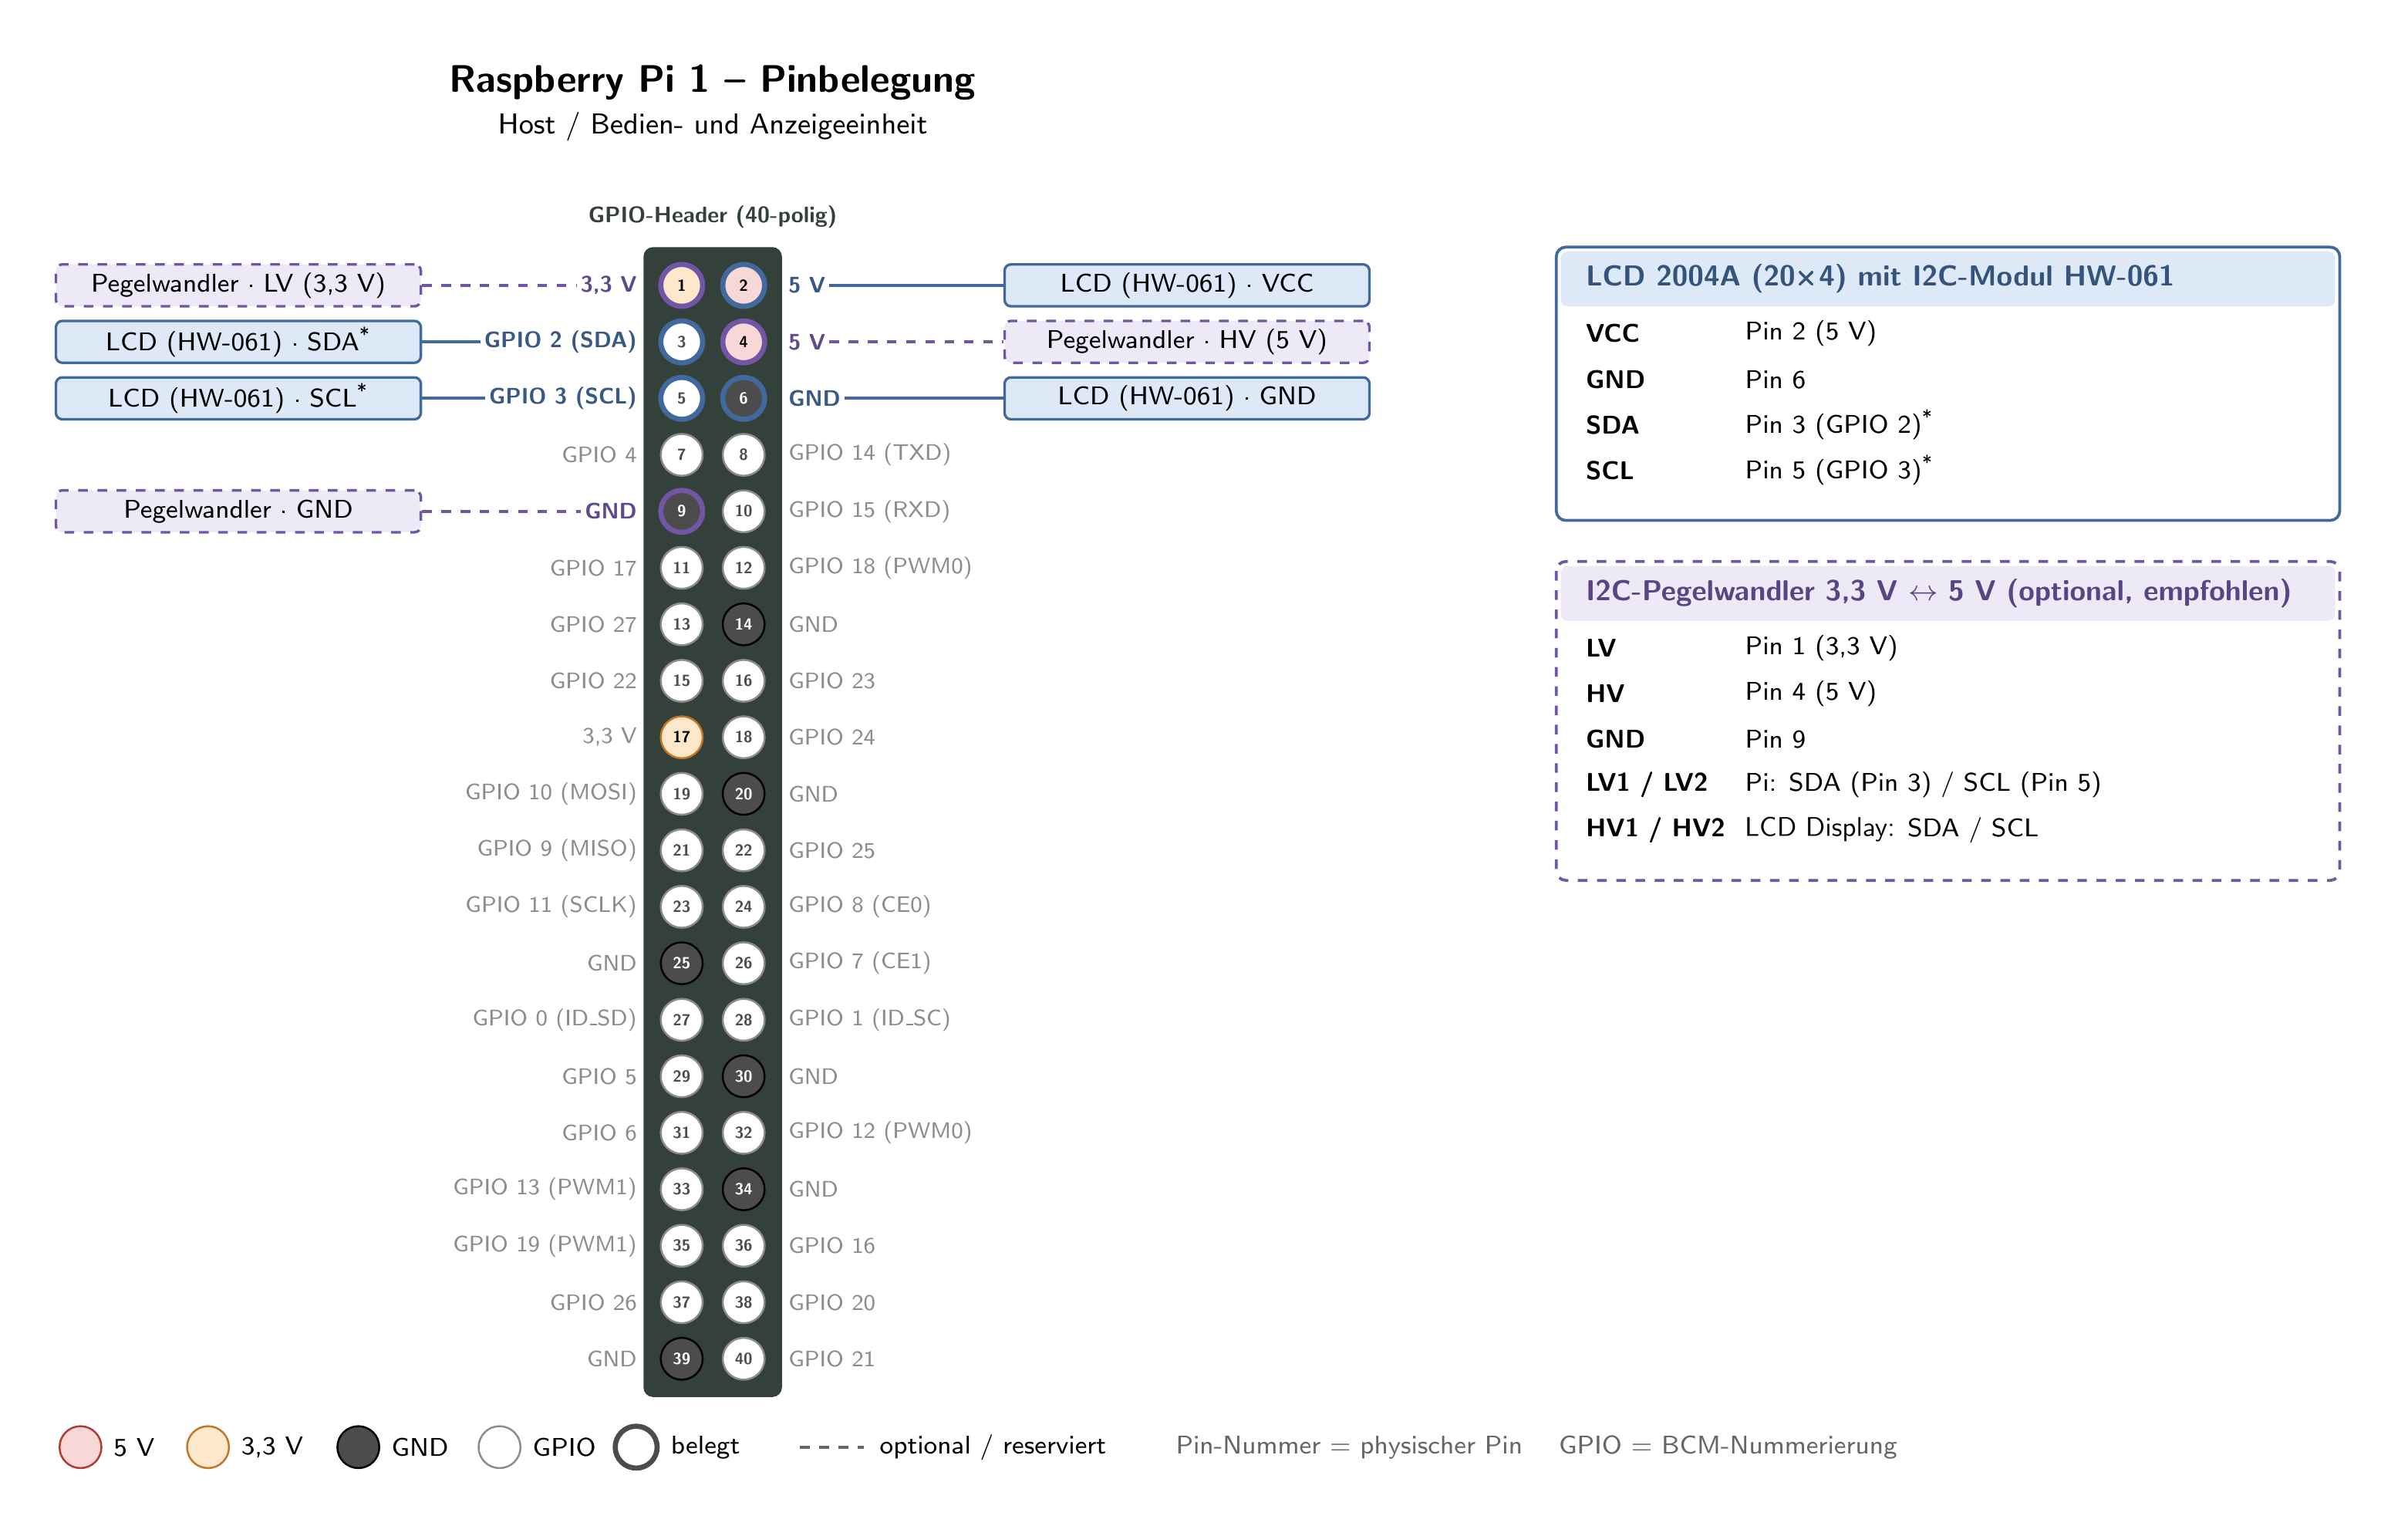
\includegraphics[width=0.8\textwidth]{images/pinout_pi1.png}
    \caption{Pinbelegung von Raspberry Pi 1}
    \label{fig:pinout_pi1}
\end{figure}

\begin{figure}[H]
    \centering
    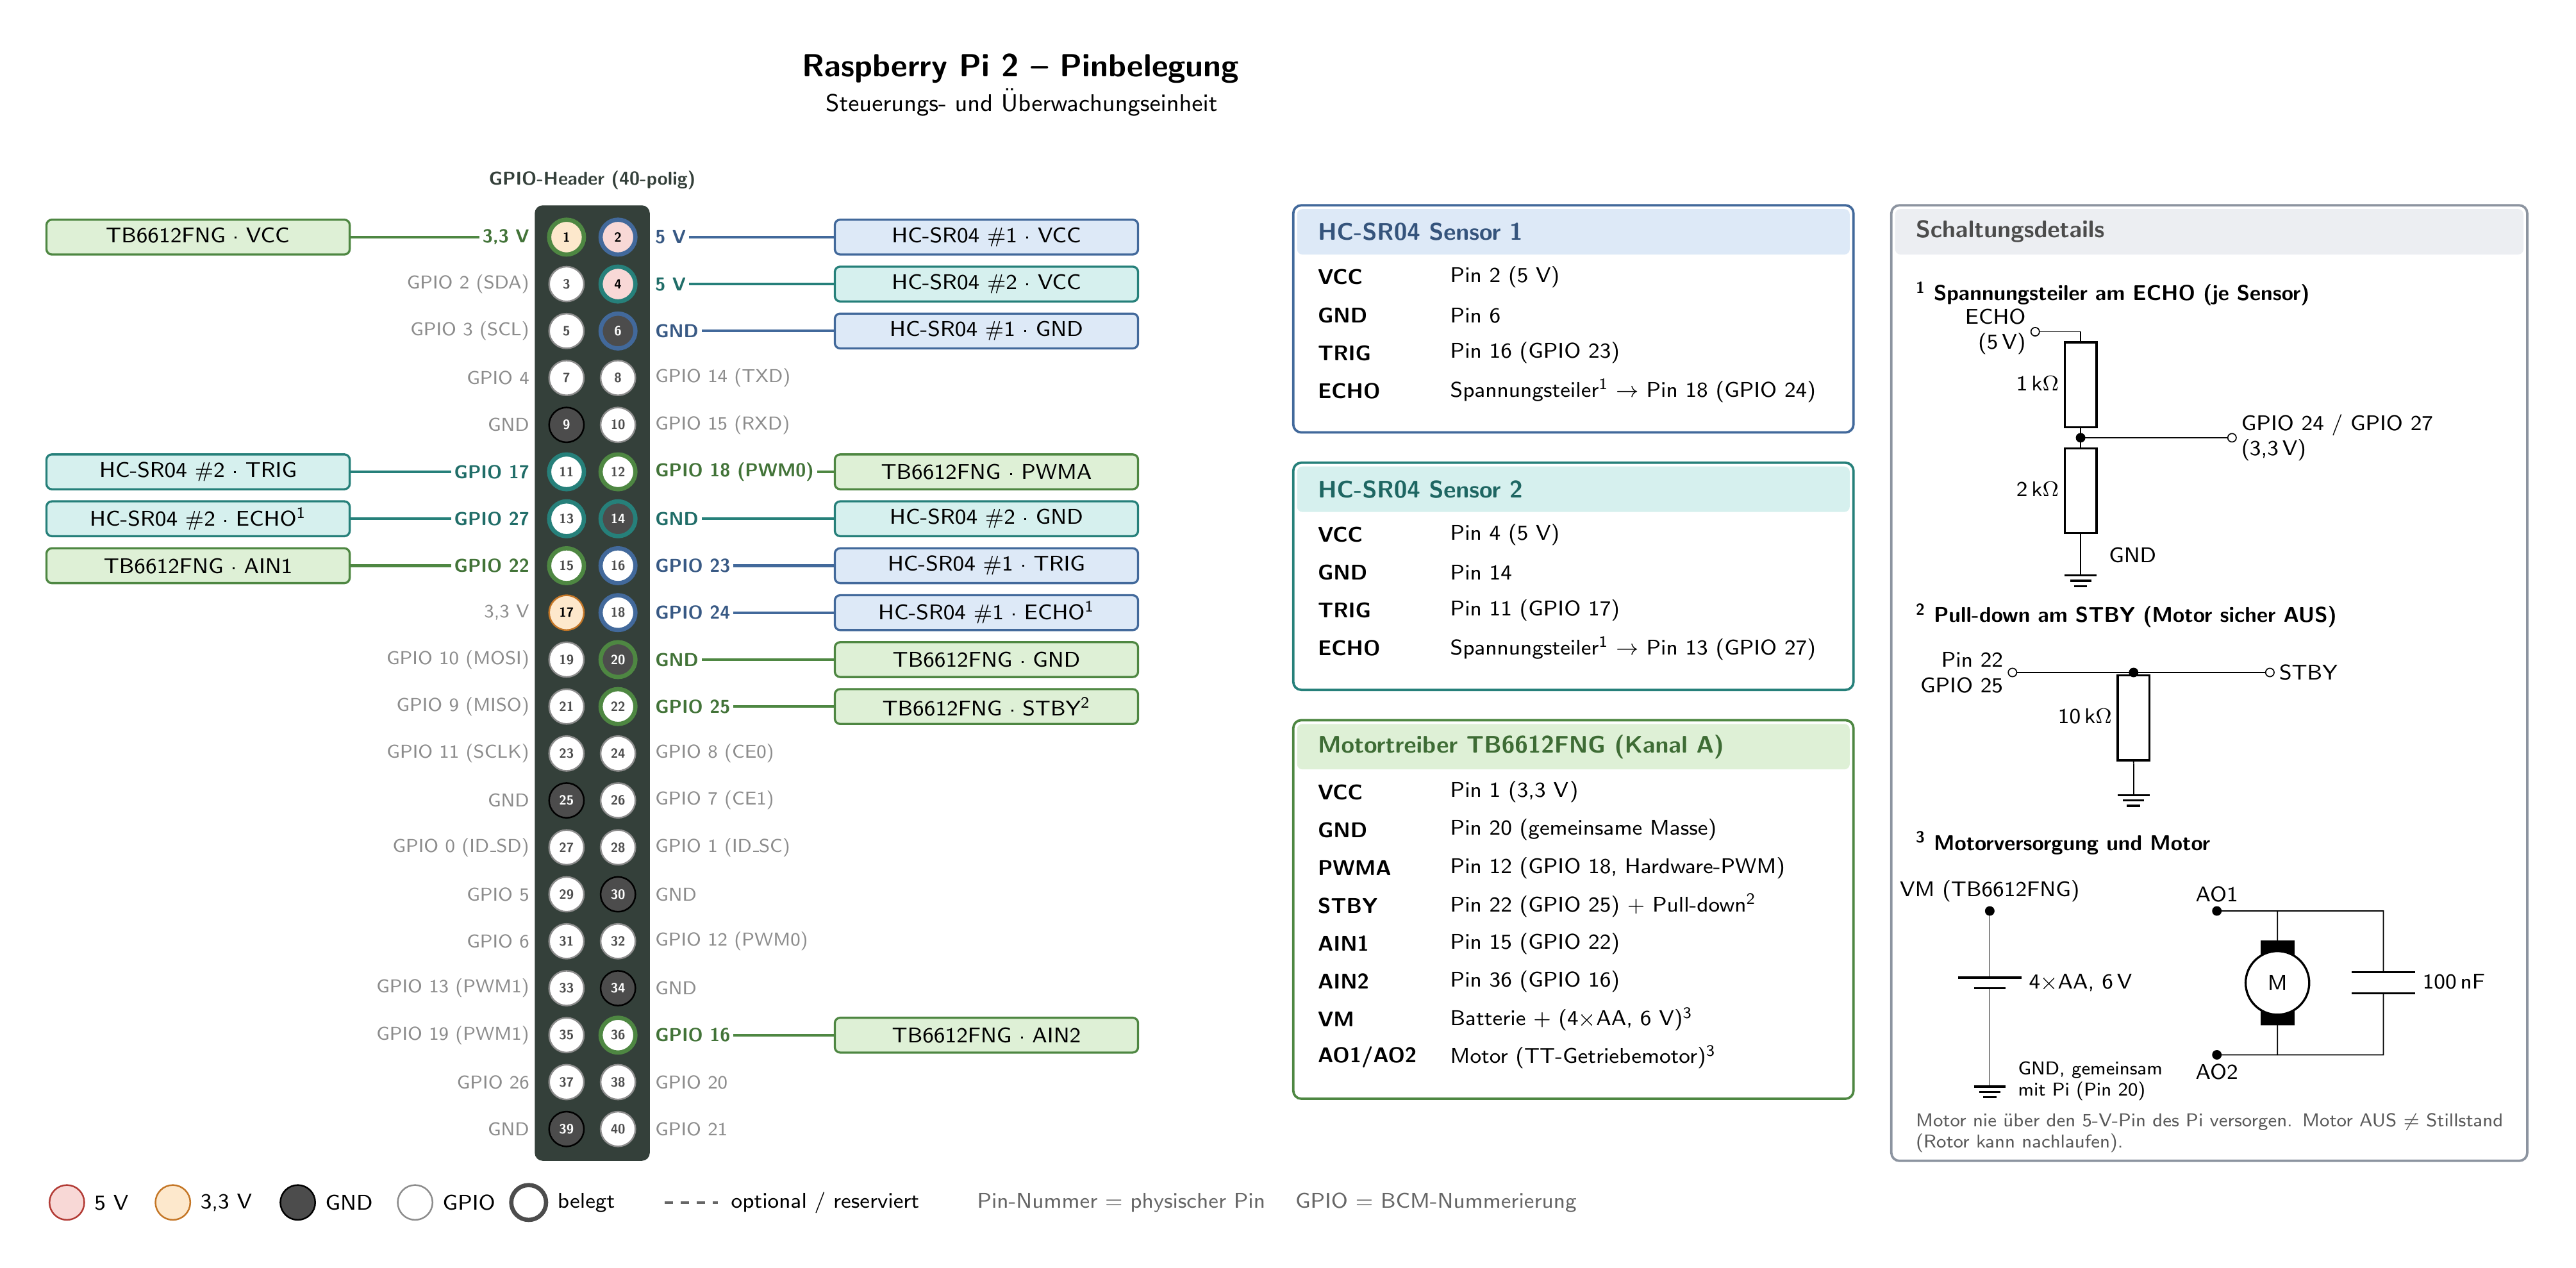
\includegraphics[width=0.8\textwidth]{images/pinout_pi2.png}
    \caption{Pinbelegung von Raspberry Pi 2}
    \label{fig:pinout_pi2}
\end{figure}
Der Link zum GitHub-Repository lautet \url{https://github.com/freudehcw/Safety_Strategies_Gruppe3}

\clearpage
\section{Programmablauf und Safety-Logik}
\label{sec:flowchart}

Abbildung~\ref{fig:flowchart} zeigt den Ablauf des Gesamtsystems. Raspberry Pi 1
übernimmt Bedienung, Anzeige, Logging und die zyklische Heartbeat-Kommunikation.
Raspberry Pi 2 führt die Sensorerfassung, Safety-Logik und Motorsteuerung aus.

\begin{figure}[H]
    \centering
    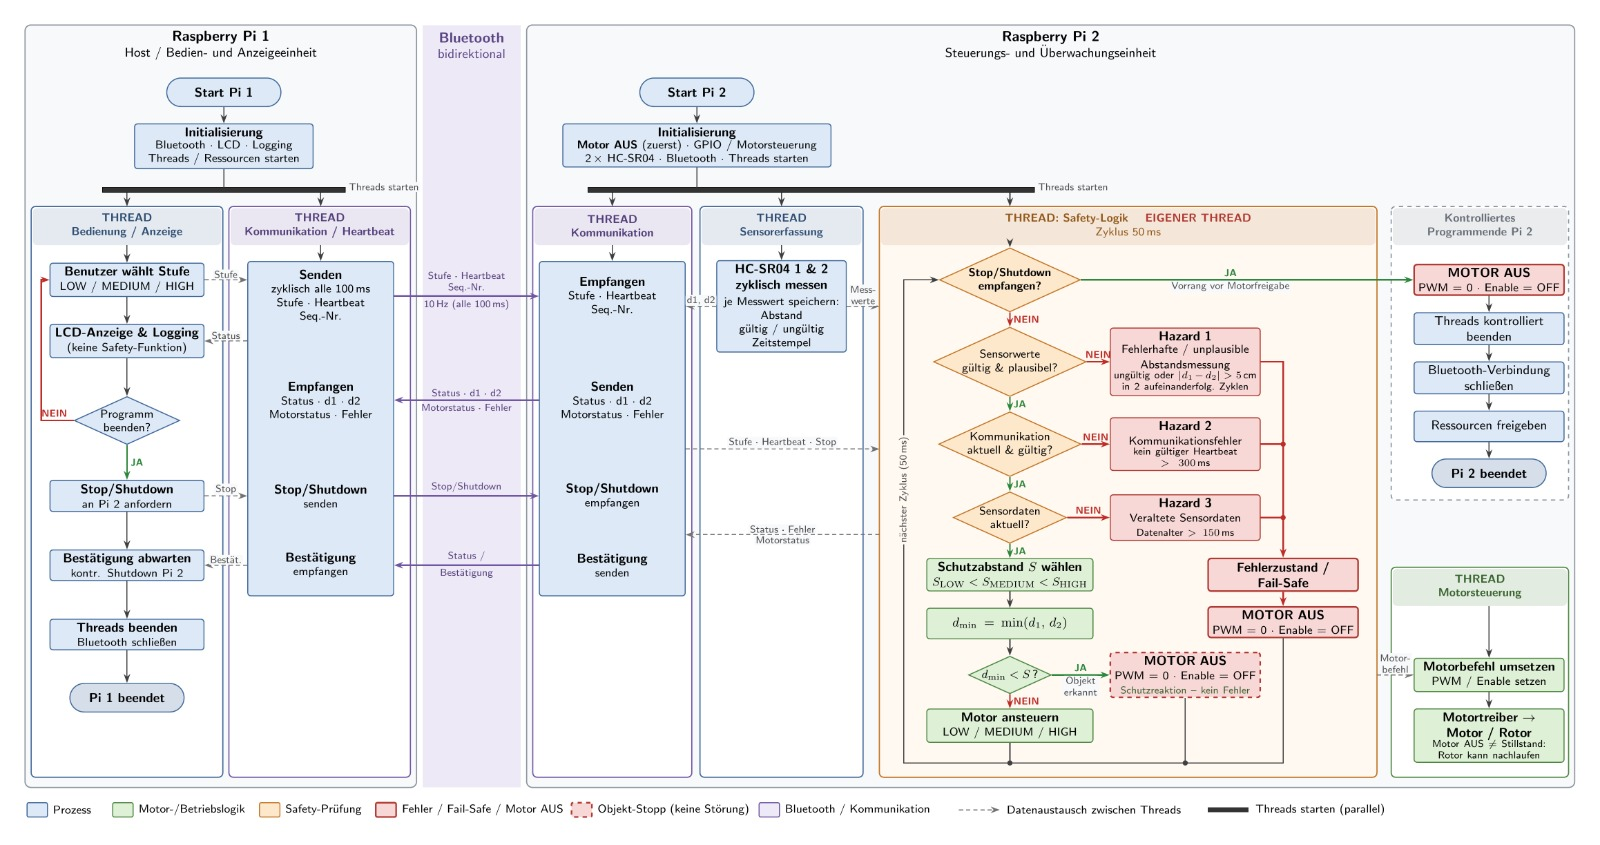
\includegraphics[width=\textwidth]{images/Campus26_Gruppe3_Flowchart_final.jpeg}
    \caption{Flussdiagramm des Gesamtsystems mit den drei adressierten Safety Hazards}
    \label{fig:flowchart}
\end{figure}

Der Safety-Logik-Thread auf Raspberry Pi 2 arbeitet zyklisch und prüft drei
Freigabebedingungen. Die Prüfungen sind logisch UND-verknüpft: Nur wenn alle drei
Bedingungen erfüllt sind, wird der Sicherheitsabstand ausgewertet und eine
Motorfreigabe ist möglich.

\begin{enumerate}
    \item \textbf{Sensorplausibilität:} Beide Sensorwerte müssen gültig sein. Eine Abweichung von mehr als 5 cm in zwei aufeinanderfolgenden Messzyklen wird als Fehler bewertet. Zusätzlich werden Messbereich und Abstandsänderung jedes Sensors geprüft (siehe Abschnitt~\ref{sec:plausibility}).
    \item \textbf{Kommunikation:} Eine gültige Nachricht bzw. ein Heartbeat muss rechtzeitig eintreffen. Bei mehr als 300 ms ohne gültige Nachricht wird der Motor abgeschaltet.
    \item \textbf{Datenaktualität:} Sensordaten dürfen höchstens 150 ms alt sein. Ältere Daten gelten als ungültig.
\end{enumerate}

Nach bestandenen Prüfungen wird der Sicherheitsabstand entsprechend der
Geschwindigkeitsstufe ausgewählt. Ist der aktuelle Abstand kleiner als der
Sicherheitsabstand, wird der Motor abgeschaltet. Andernfalls darf der Motor mit
der freigegebenen Stufe betrieben werden.

Nach jedem Zyklus beginnt die Prüfung von vorn. Fehler und Objekt-Stopp sind
daher nicht selbsthaltend: Sind im nächsten Zyklus alle Bedingungen erfüllt,
läuft der Motor ohne Quittierung wieder an (Wiederanlaufbedingung, siehe
Abschnitt~\ref{sec:states}).

Das Programmende ist ebenfalls Teil des Ablaufs. Ein Stop/Shutdown-Befehl von
Raspberry Pi 1 führt auf Raspberry Pi 2 zuerst zu Motor AUS und anschließend zum
kontrollierten Beenden des Programms.

\section{Safety Hazards}
\label{sec:hazards}

Für den Demonstrator werden sechs zentrale Safety Hazards betrachtet. Drei davon
werden durch konkrete Maßnahmen im Design adressiert. Drei weitere werden bewusst
nicht vollständig adressiert, weil dafür zusätzliche unabhängige oder
sicherheitsgerichtete Hardware erforderlich wäre.

\keybox{Sicherer Zustand: Motor AUS -- der Rotor wird nicht aktiv angetrieben.}

\subsection{Übersicht}

\begin{table}[H]
    \centering
    \small
    \begin{tabularx}{\textwidth}{@{}p{0.7cm}p{2.6cm}YY@{}}
        \toprule
        \textbf{ID} & \textbf{Status} & \textbf{Hazard} & \textbf{Umgang im Projekt} \\
        \midrule
        H1 & Adressiert & Motor läuft weiter, obwohl ein Objekt zu nahe ist, weil ein Sensorwert falsch oder ungültig ist. & Gültigkeitsprüfung, Vergleich beider Sensoren, 5-cm-Plausibilitätsgrenze; bei Fehler Motor AUS. \\
        H2 & Adressiert & Motor arbeitet mit einem veralteten oder ungültigen Geschwindigkeitsbefehl weiter. & 10-Hz-Heartbeat, Sequenznummer und 300-ms-Timeout; bei Kommunikationsfehler Motor AUS. \\
        H3 & Adressiert & Motor läuft weiter, obwohl veraltete Sensordaten verwendet werden. & Zeitstempel je Messwert, maximales Datenalter 150 ms; bei Überschreitung Motor AUS. \\
        H4 & Nicht vollständig adressiert & Rotor läuft trotz angefordertem STOP weiter oder kommt zu spät zum Stillstand. & Software setzt PWM = 0 und Enable = OFF; Nachlauf wird berücksichtigt, Defekt der Leistungsstufe bleibt offen. \\
        H5 & Nicht vollständig adressiert & Tatsächliche Motordrehzahl ist höher als vom System angenommen. & Keine unabhängige Drehzahlmessung; konservative Geschwindigkeitsklassen und Schutzabstände. \\
        H6 & Nicht vollständig adressiert & Beide HC-SR04 liefern gleichzeitig ähnliche falsche Werte. & Quervergleich erkennt Common-Cause-Fehler nicht sicher; Grenze wird dokumentiert. \\
        \bottomrule
    \end{tabularx}
    \caption{Zentrale Safety Hazards des Demonstrators}
\end{table}

\subsection{Adressierte Hazards}

\subsubsection{H1 -- Fehlerhafte oder unplausible Abstandsmessung}
\label{haz:h1}

\hazfield{Hazard}
Der Motor läuft weiter, obwohl sich ein Objekt bereits innerhalb des erforderlichen Sicherheitsabstands befindet.

\hazfield{Ursache}
Ein Sensor liefert keinen Wert, einen zu großen Wert oder einen deutlich anderen Wert als der zweite Sensor.

\hazfield{Erkennung und Maßnahme}
Beide HC-SR04 müssen einen gültigen Messwert liefern. Die absolute Differenz der
beiden Werte wird geprüft. Ist
\[
    |d_1-d_2| > 5\,\mathrm{cm}
\]
in zwei aufeinanderfolgenden Messzyklen, gelten die Sensoren als unplausibel.
Ein fehlender oder ungültiger Messwert wird ebenfalls als Fehler behandelt.
Für die Abstandsentscheidung wird der kleinere der beiden gültigen Werte
verwendet.

\hazfield{Fail-Safe-Reaktion}
\failsafe{Ungültige oder unplausible Sensordaten $\rightarrow$ Motor AUS}

\hazfield{Test}
Einen Sensor verdecken, gezielt einen abweichenden Messwert erzeugen oder per
Testmodus einspeisen. Der Fehler muss erkannt werden und der Motor muss
abschalten.

\subsubsection{H2 -- Kommunikationsfehler zwischen Raspberry Pi 1 und Raspberry Pi 2}
\label{haz:h2}

\hazfield{Hazard}
Der Motor arbeitet mit einem alten oder ungültigen Geschwindigkeitsbefehl weiter.

\hazfield{Ursache}
Bluetooth-Verbindung unterbrochen, Pi 1 ausgefallen, Nachricht verspätet oder
Nachrichteninhalt ungültig.

\hazfield{Erkennung und Maßnahme}
Pi 1 sendet alle 100 ms einen Heartbeat zusammen mit dem aktuellen Befehl. Pi 2
prüft Wertebereich und Sequenznummer. Trifft länger als 300 ms keine gültige
Nachricht ein, wird ein Kommunikationsfehler gesetzt. Damit entsprechen drei
ausbleibende Heartbeats dem Timeout.

\hazfield{Fail-Safe-Reaktion}
\failsafe{Kommunikationsfehler oder Timeout $\rightarrow$ Motor AUS}

\hazfield{Test}
Während des Motorbetriebs die Bluetooth-Verbindung trennen oder das Pi-1-Programm
anhalten. Spätestens nach dem definierten Timeout muss Pi 2 den Motor
abschalten.

\subsubsection{H3 -- Veraltete Sensordaten}
\label{haz:h3}

\hazfield{Hazard}
Die Safety-Entscheidung wird mit einem Abstandswert getroffen, der nicht mehr den
aktuellen Zustand beschreibt.

\hazfield{Ursache}
Ein Sensor-Thread hängt, wird verspätet ausgeführt oder aktualisiert seine Daten
nicht mehr.

\hazfield{Erkennung und Maßnahme}
Jeder Messwert wird mit einem monotonen Zeitstempel gespeichert. Vor der
Verwendung prüft der Safety-Logik-Thread das Alter. Messwerte älter als 150 ms
gelten als ungültig und dürfen keine Motorfreigabe bewirken.

\hazfield{Fail-Safe-Reaktion}
\failsafe{Sensordaten zu alt $\rightarrow$ Motor AUS}

\hazfield{Test}
Einen Sensor-Thread im Testmodus länger als 150 ms blockieren. Der Safety-Thread
muss den veralteten Messwert erkennen und den Motor abschalten.

\subsection{Nicht vollständig adressierte Hazards}

\subsubsection{H4 -- Motor oder Motortreiber reagiert nicht korrekt auf STOP}
\label{haz:h4}

\hazfield{Hazard}
Der Rotor wird trotz angeforderter Abschaltung weiter angetrieben oder kommt erst
verspätet zum Stillstand.

\hazfield{Warum relevant}
Ein Software-Stoppkommando garantiert weder eine funktionierende
Leistungselektronik noch sofortigen mechanischen Stillstand.

\hazfield{Warum nicht vollständig adressiert}
Die vorhandene Architektur besitzt keinen unabhängigen sicherheitsgerichteten
Abschaltpfad und keine Rückmeldung, ob der Rotor tatsächlich steht.

\hazfield{Maßnahme im Demonstrator}
PWM und Enable werden deaktiviert. Die Nachlaufzeit des Rotors wird am realen
Aufbau gemessen und bei der Wahl der Sicherheitsabstände berücksichtigt.

\hazfield{Industrielle Lösung}
Unabhängige sicherheitsgerichtete Abschaltung, beispielsweise geeigneter
Safety-Controller, Sicherheitsrelais oder ein Antrieb mit Safe-Torque-Off.

\subsubsection{H5 -- Tatsächliche Motordrehzahl ist unbekannt}
\label{haz:h5}

\hazfield{Hazard}
Der Rotor dreht schneller, als es die gewählte Geschwindigkeitsstufe vermuten
lässt.

\hazfield{Warum relevant}
PWM-Prozent und reale Motordrehzahl sind nicht gleichzusetzen. Last,
Versorgungsspannung und Motoreigenschaften beeinflussen die tatsächliche
Drehzahl und Nachlaufzeit.

\hazfield{Warum nicht vollständig adressiert}
Es ist kein unabhängiger Encoder oder anderer Drehzahlsensor vorhanden.

\hazfield{Maßnahme im Demonstrator}
Es werden nur die Klassen \texttt{LOW}, \texttt{MEDIUM} und \texttt{HIGH}
verwendet. Für höhere Stufen wird ein größerer, konservativ festgelegter
Sicherheitsabstand verwendet.

\hazfield{Industrielle Lösung}
Unabhängige Drehzahlerfassung mit sicherheitsgerichteter Auswertung.

\subsubsection{H6 -- Gemeinsamer Fehler beider Abstandssensoren}
\label{haz:h6}

\hazfield{Hazard}
Beide HC-SR04 liefern gleichzeitig ähnliche, aber falsche Abstandswerte.

\hazfield{Warum relevant}
Beide Sensoren verwenden dasselbe Messprinzip. Ungünstige Oberflächen, Winkel,
Reflexionen oder gemeinsame Störungen können daher beide Sensoren ähnlich
beeinflussen.

\hazfield{Warum nicht vollständig adressiert}
Ein Vergleich zweier gleicher Sensoren erkennt nur Unterschiede zwischen den
Messwerten. Sind beide Werte durch dieselbe Ursache falsch, kann die
Plausibilitätsprüfung erfolgreich sein, obwohl der reale Abstand gefährlich
klein ist.

\hazfield{Maßnahme im Demonstrator}
Die Sensoren werden zeitlich versetzt angesteuert und die Einschränkung des
Quervergleichs wird ausdrücklich dokumentiert.

\hazfield{Industrielle Lösung}
Geeignete sicherheitsgerichtete Sensorik und je nach Anwendung diversitäre
Messprinzipien.

\clearpage
\section{Security-Betrachtung}
\label{sec:security}

Die Security-Betrachtung konzentriert sich auf die Bluetooth-Kommunikation
zwischen den beiden Raspberry Pis. Die lokale Abstandsauswertung auf Raspberry
Pi 2 bleibt auch dann aktiv, wenn die Funkverbindung gestört oder unterbrochen
wird. Security-Maßnahmen dürfen daher nicht die Fail-Safe-Reaktion verhindern.
Drei Bedrohungen werden durch konkrete Maßnahmen im Design adressiert. Drei
weitere werden bewusst nicht vollständig adressiert, weil dafür zusätzliche
Hardware- oder Plattformmaßnahmen erforderlich wären.

\subsection{Übersicht}

\begin{table}[H]
    \centering
    \small
    \begin{tabularx}{\textwidth}{@{}p{0.8cm}p{3.5cm}YY@{}}
        \toprule
        \textbf{ID} & \textbf{Bedrohung} & \textbf{Mögliche Auswirkung} & \textbf{Maßnahme im Demonstrator} \\
        \midrule
        T1 & Unberechtigtes Gerät sendet Befehle & Falsche Geschwindigkeitsstufe oder unerwünschte Bedienung & Bluetooth-Pairing/Bonding; Pi 2 akzeptiert nur den vorgesehenen Kommunikationspartner; Nachrichteninhalt wird geprüft. \\
        T2 & Alte oder doppelte Nachricht wird erneut verarbeitet & Veralteter Befehl könnte erneut wirksam werden & Sequenznummer je Nachricht; alte und doppelte Nachrichten werden verworfen. \\
        T3 & Bluetooth wird gestört oder fällt aus & Pi 2 erhält keine aktuellen Befehle mehr & Heartbeat und 300-ms-Timeout; bei Kommunikationsverlust Motor AUS. Verfügbarkeit kann dadurch verloren gehen, Safety bleibt erhalten. \\
        \midrule
        T4 & Kompromittierter Raspberry Pi 1 sendet formal gültige, aber manipulierte Befehle & Unerwünschte Geschwindigkeitsstufe, falsche Statusanzeige für den Bediener & \textit{Nicht vollständig adressiert.} Pi 2 entscheidet lokal über die Abschaltung; der Sicherheitsabstand gilt für jede Stufe. \\
        T5 & Manipulation von Software oder Konfiguration auf Pi 2 & Grenzwerte, Timeouts oder Sicherheitsabstände werden verändert oder die Safety-Logik deaktiviert & \textit{Nicht vollständig adressiert.} Konstanten zentral definiert und über Git versioniert; kein Schutz am laufenden Gerät. \\
        T6 & Akustische Störung oder Spoofing der HC-SR04 & Beide Sensoren liefern gleichzeitig falsche Abstände & \textit{Nicht vollständig adressiert.} Plausibilitätsprüfung und zeitversetztes Triggern; gleichartige Manipulation beider Sensoren wird nicht sicher erkannt. \\
        \bottomrule
    \end{tabularx}
    \caption{Security-Bedrohungen und Gegenmaßnahmen}
    \label{tab:security-threats}
\end{table}

\subsection{Adressierte Bedrohungen}

\subsubsection*{T1 -- Unberechtigtes Gerät sendet Befehle}

\textbf{Bedrohung:} Ein fremdes Bluetooth-Gerät baut eine Verbindung zu
Raspberry Pi 2 auf und sendet Steuerbefehle.

\textbf{Angriffsweg:} Ein Angreifer in Funkreichweite gibt sich als
Kommunikationspartner aus oder sendet selbst erzeugte Nachrichten mit
unzulässigem Inhalt.

\textbf{Erkennung und Maßnahme:} Pi 2 akzeptiert nur Verbindungen des
gepaarten bzw.\ gebondeten Raspberry Pi 1. Jede eingehende Nachricht wird vor
der Verwendung auf Nachrichtentyp, Länge und gültigen Wertebereich geprüft.
Nur die Stufen LOW, MEDIUM und HIGH werden als Befehl akzeptiert; unbekannte
Werte führen nicht zu einem Default-Betrieb.

\textbf{Reaktion:}
\begin{center}
    Unbekannter Absender oder ungültiger Nachrichteninhalt $\rightarrow$ Nachricht verwerfen, keine Motorfreigabe
\end{center}

\textbf{Test:} Verbindungsversuch mit einem nicht gepaarten Gerät durchführen
sowie im Testmodus Nachrichten mit falschem Typ, falscher Länge oder
unzulässiger Stufe einspeisen. Die Verbindung bzw.\ Nachricht muss abgelehnt
werden; der Motorzustand darf sich dadurch nicht ändern.

\subsubsection*{T2 -- Wiedereinspielen alter oder doppelter Nachrichten}

\textbf{Bedrohung:} Eine zuvor gültige Nachricht wird erneut verarbeitet und
ein veralteter Befehl wird dadurch wieder wirksam.

\textbf{Angriffsweg:} Aufgezeichnete Nachrichten werden erneut gesendet
(Replay), oder Nachrichten treffen durch Übertragungsfehler doppelt bzw.\ in
falscher Reihenfolge ein.

\textbf{Erkennung und Maßnahme:} Jede Steuerungsnachricht von Pi 1 trägt eine
fortlaufende Sequenznummer. Pi 2 speichert die zuletzt akzeptierte
Sequenznummer und verwirft Nachrichten mit gleicher oder älterer Nummer. Eine
verworfene Nachricht gilt nicht als gültiger Heartbeat und kann den
300-ms-Timeout daher nicht zurücksetzen.

\textbf{Reaktion:}
\begin{center}
    Alte oder doppelte Sequenznummer $\rightarrow$ Nachricht verwerfen; bleibt eine gültige Nachricht aus $\rightarrow$ Motor AUS
\end{center}

\textbf{Test:} Im Testmodus eine bereits verarbeitete Nachricht erneut senden
und Nachrichten mit veralteter Sequenznummer einspeisen. Die Nachrichten
dürfen keinen Befehl auslösen; bei ausschließlich veralteten Nachrichten muss
der Motor nach spätestens 300\,ms abschalten.

\subsubsection*{T3 -- Störung oder Ausfall der Bluetooth-Verbindung}

\textbf{Bedrohung:} Raspberry Pi 2 erhält keine aktuellen Befehle mehr und
könnte mit einem veralteten Befehl weiterarbeiten.

\textbf{Angriffsweg:} Gezielte Funkstörung (Jamming), Unterbrechung der
Verbindung oder Ausfall von Pi 1.

\textbf{Erkennung und Maßnahme:} Pi 1 sendet alle 100\,ms einen Heartbeat mit
dem aktuellen Befehl. Pi 2 überwacht mit einer monotonen Uhr den Zeitpunkt der
letzten gültigen Nachricht. Trifft länger als 300\,ms keine gültige Nachricht
ein, wird ein Kommunikationsfehler gesetzt. Die lokale Abstandsauswertung auf
Pi 2 bleibt dabei unabhängig von der Funkverbindung aktiv.

\textbf{Reaktion:}
\begin{center}
    Kein gültiger Heartbeat innerhalb von 300\,ms $\rightarrow$ Motor AUS
\end{center}

Der Angriff kann damit die Verfügbarkeit des Demonstrators beeinträchtigen,
führt aber nicht zu einem unsicheren Zustand.

\textbf{Test:} Während des Motorbetriebs die Bluetooth-Verbindung trennen oder
das Programm auf Pi 1 anhalten (vgl.\ TC-03). Spätestens nach 300\,ms muss Pi 2
den Motor abschalten.

\subsection{Nicht vollständig adressierte Bedrohungen}

\subsubsection*{T4 -- Kompromittierter Raspberry Pi 1}

\textbf{Bedrohung:} Ein Angreifer erlangt Kontrolle über Raspberry Pi 1 und
sendet Nachrichten, die Typ-, Längen-, Wertebereichs- und Sequenzprüfung
bestehen, inhaltlich aber nicht dem Willen des Bedieners entsprechen.

\textbf{Warum relevant:} Pairing/Bonding und Sequenznummern stellen nur sicher,
dass eine Nachricht vom vorgesehenen Gerät stammt. Sie sagen nichts darüber
aus, ob dieses Gerät vertrauenswürdig arbeitet. Zusätzlich kann ein
manipulierter Pi 1 dem Bediener am LCD einen falschen Systemzustand anzeigen.

\textbf{Warum nicht vollständig adressiert:} Es gibt keine Integritätsprüfung
der Software auf Pi 1 und keine unabhängige Bedienerbestätigung auf Pi 2.

\textbf{Maßnahme im Demonstrator:} Die Abstandsüberwachung läuft lokal auf
Pi 2 und kann durch Befehle von Pi 1 nicht deaktiviert werden. Auch bei
manipulierter Stufe gilt der zugehörige Sicherheitsabstand. Die Auswirkung
beschränkt sich damit im Wesentlichen auf Verfügbarkeit und
Bedienerinformation.

\textbf{Industrielle Lösung:} Secure Boot, gehärtetes Betriebssystem,
Ende-zu-Ende-authentifizierte Nachrichten sowie eine unabhängige Statusanzeige
bzw.\ ein Not-Halt direkt an der Maschine.

\subsubsection*{T5 -- Manipulation von Software oder Konfiguration auf Raspberry Pi 2}

\textbf{Bedrohung:} Durch physischen Zugriff, beispielsweise durch Austausch
der SD-Karte, oder durch Zugriff auf das Betriebssystem werden Programm oder
Parameter von Pi 2 verändert.

\textbf{Warum relevant:} Pi 2 trägt die gesamte Safety-Entscheidung. Eine
Änderung der Sicherheitsabstände, des 300-ms-Timeouts oder der
Plausibilitätsgrenze hebelt die Maßnahmen gegen H1--H3 direkt aus, ohne dass
dies von außen erkennbar ist.

\textbf{Warum nicht vollständig adressiert:} Der Raspberry Pi 4B besitzt im
Projektaufbau keine verifizierte Boot-Kette und keinen Schutz der
Speichermedien. Ein Angreifer mit physischem Zugriff liegt außerhalb des
Projektumfangs (siehe Abschnitt~\ref{subsec:security-abgrenzung}).

\textbf{Maßnahme im Demonstrator:} Safety-relevante Konstanten sind zentral
definiert, Änderungen werden über Git versioniert und vor dem Merge geprüft.
Damit ist der Soll-Stand nachvollziehbar; der Ist-Stand am Gerät wird jedoch
nicht überprüft.

\textbf{Industrielle Lösung:} Secure Boot mit signierter Firmware,
schreibgeschützte bzw.\ verschlüsselte Parameter, Zugriffsschutz am Gehäuse
und Prüfsummen über Safety-Parameter beim Start.

\subsubsection*{T6 -- Akustische Störung oder Spoofing der Ultraschallsensoren}

\textbf{Bedrohung:} Ein Angreifer stört die HC-SR04 gezielt mit Ultraschall
im Bereich von 40\,kHz oder erzeugt künstliche Echos.

\textbf{Warum relevant:} Beide Sensoren arbeiten mit demselben Messprinzip und
derselben Frequenz. Eine externe Quelle kann daher beide gleichzeitig
beeinflussen. Je nach Angriff entstehen zu kleine Messwerte (unnötiges
Abschalten, Verlust der Verfügbarkeit) oder Messwerte, die ein tatsächlich
nahes Objekt verdecken.

\textbf{Warum nicht vollständig adressiert:} Der Quervergleich erkennt nur
Unterschiede zwischen den Sensoren. Werden beide gleichartig manipuliert,
besteht die Plausibilitätsprüfung. Es handelt sich um einen vorsätzlich
herbeigeführten Common-Cause-Fehler (vgl.\ H6).

\textbf{Maßnahme im Demonstrator:} Zeitversetztes Triggern, Gültigkeits- und
Plausibilitätsprüfung sowie Verwendung des kleineren Messwerts. Die
Einschränkung wird ausdrücklich dokumentiert.

\textbf{Industrielle Lösung:} Diversitäre Sensorik, beispielsweise Ultraschall
kombiniert mit Lichtvorhang oder Safety-Laserscanner, codierte Messsignale und
physische Schutzeinrichtungen.

\subsection{Abgrenzung}
\label{subsec:security-abgrenzung}

Der Demonstrator implementiert kein eigenes kryptographisches Protokoll und
keinen vollständigen Schutz gegen einen kompromittierten Raspberry Pi oder
gezieltes Funk-Jamming. Ein Angreifer mit physischem Zugriff auf das Gerät oder
auf das Betriebssystem liegt außerhalb des Projektumfangs. Entscheidend für das
Safety-Konzept ist, dass fehlerhafte oder ausbleibende Kommunikation keine
Motorfreigabe aufrechterhält.

\clearpage
\section{Anforderungen und Tests}
\label{sec:requirements}

Die Anforderungen sind bewusst auf die für den Demonstrator wesentlichen
Punkte beschränkt. Zeit- und Grenzwerte sind Design-Startwerte und müssen am
realen Aufbau verifiziert werden.

\subsection{Safety-Anforderungen}

\begin{table}[H]
    \centering
    \small
    \begin{tabularx}{\textwidth}{@{}p{1.5cm}Yp{2.0cm}@{}}
        \toprule
        \textbf{ID} & \textbf{Anforderung} & \textbf{Bezug} \\
        \midrule
        SAF-01 & Der sichere Zustand des Systems ist Motor AUS. Auf Pi 2 bedeutet dies PWM = 0 und Enable = OFF. & H1--H6 \\
        SAF-02 & Pi 2 muss beim Programmstart im sicheren Zustand bleiben, bis Initialisierung, Sensorprüfung und Kommunikation gültig sind. & H1--H3 \\
        SAF-03 & Beide Abstandssensoren müssen gültige Werte liefern. Eine Abweichung größer 5 cm in zwei aufeinanderfolgenden Messzyklen muss zu Motor AUS führen. & H1 \\
        SAF-04 & Jeder Sensormesswert muss einen Zeitstempel besitzen. Daten älter als 150 ms dürfen keine Motorfreigabe bewirken. & H3 \\
        SAF-05 & Pi 1 muss alle 100 ms einen Heartbeat senden. Erhält Pi 2 länger als 300 ms keine gültige Nachricht, muss der Motor abgeschaltet werden. & H2 \\
        SAF-06 & Der Safety-Logik-Thread auf Pi 2 soll zyklisch alle 50 ms laufen und die Safety-Bedingungen vor einer Motorfreigabe prüfen. & H1--H3 \\
        SAF-07 & Nur die gültigen Geschwindigkeitsstufen LOW, MEDIUM und HIGH dürfen verwendet werden. Für jede Stufe muss ein definierter Sicherheitsabstand existieren. & H5 \\
        SAF-08 & Unterschreitet der aktuelle gültige Abstand den Sicherheitsabstand der gewählten Stufe, muss der Motor abgeschaltet werden. & H1, H5 \\
        SAF-09 & Ein Stop/Shutdown-Befehl muss auf Pi 2 zuerst Motor AUS auslösen. Erst danach dürfen Threads und Programm beendet werden. & H4 \\
        SAF-10 & Die endgültigen Sicherheitsabstände müssen am realen Aufbau anhand der beobachteten Reaktions- und Nachlaufzeiten festgelegt und dokumentiert werden. & H4, H5 \\
        \bottomrule
    \end{tabularx}
    \caption{Safety-Anforderungen}
\end{table}

\subsection{Security-Anforderungen}

\begin{table}[H]
    \centering
    \small
    \begin{tabularx}{\textwidth}{@{}p{1.5cm}Y@{}}
        \toprule
        \textbf{ID} & \textbf{Anforderung} \\
        \midrule
        SEC-01 & Die Bluetooth-Verbindung soll nur mit dem vorgesehenen, gepaarten bzw. gebondeten Kommunikationspartner aufgebaut werden. \\
        SEC-02 & Eingehende Nachrichten müssen vor der Verwendung auf Typ, Länge und gültigen Wertebereich geprüft werden. \\
        SEC-03 & Jede Steuerungsnachricht muss eine Sequenznummer tragen. Alte oder doppelte Nachrichten dürfen nicht erneut ausgeführt werden. \\
        SEC-04 & Ein Kommunikationsangriff oder Kommunikationsausfall darf die lokale Abstandsauswertung auf Pi 2 nicht deaktivieren; bei Timeout gilt Motor AUS. \\
        \bottomrule
    \end{tabularx}
    \caption{Security-Anforderungen}
\end{table}

\subsection{Unterstützende Anforderungen}

\begin{itemize}
    \item Das LCD zeigt Systemzustand, Abstände, Geschwindigkeitsstufe und Fehler an. Das LCD ist keine Safety-Funktion.
    \item Logging protokolliert wichtige Zustands- und Fehlerereignisse. Logging ist keine Risikominderung und darf den Safety-Logik-Thread nicht blockieren.
    \item Gemeinsame Daten zwischen Threads müssen konsistent übertragen werden, beispielsweise über Mutex und Snapshot-Kopie.
    \item Änderungen an Safety-relevanter Software werden über Git versioniert und sollen vor dem Merge überprüft werden.
\end{itemize}

\subsection{Geplante Tests}

\begin{table}[H]
    \centering
    \small
    \begin{tabularx}{\textwidth}{@{}p{1.5cm}YY@{}}
        \toprule
        \textbf{Test} & \textbf{Durchführung} & \textbf{Erwartetes Ergebnis} \\
        \midrule
        TC-01 & Einen Sensor verdecken oder ungültigen Messwert erzeugen. & Sensorfehler wird erkannt; Motor AUS. \\
        TC-02 & Zwei Sensorwerte um mehr als 5 cm abweichen lassen. & Nach zwei aufeinanderfolgenden unplausiblen Messzyklen Motor AUS. \\
        TC-03 & Bluetooth-Verbindung während des Motorbetriebs trennen oder Pi 1 anhalten. & Spätestens nach 300 ms ohne gültige Nachricht wird die Motorfreigabe entzogen. \\
        TC-04 & Sensor-Thread länger als 150 ms blockieren. & Daten werden als veraltet erkannt; Motor AUS. \\
        TC-05 & Testobjekt in den Sicherheitsabstand der jeweiligen Geschwindigkeitsstufe bewegen. & Motor wird abgeschaltet, sobald der gültige Abstand kleiner als der konfigurierte Sicherheitsabstand ist. \\
        TC-06 & Programmende auf Pi 1 auslösen. & Pi 1 sendet Stop/Shutdown; Pi 2 setzt zuerst Motor AUS und beide Programme beenden kontrolliert. \\
        \bottomrule
    \end{tabularx}
    \caption{Geplante System- und Safety-Tests}
\end{table}


\end{document}
